\documentclass[10pt,xcolor=dvipsnames]{beamer}

\usetheme[progressbar=frametitle]{metropolis}
\usepackage{appendixnumberbeamer}

\usepackage{booktabs}
\usepackage[scale=2]{ccicons}

\usepackage{pgfplots}
\usepgfplotslibrary{dateplot}

\usepackage{xspace}
\newcommand{\themename}{\textbf{\textsc{metropolis}}\xspace}

\usepackage{pdfpages}
\setbeamercolor{section title}{fg=Blue,bg=Blue}
\setbeamercolor*{structure}{bg=Blue!20,fg=Blue}
\setbeamercolor*{palette primary}{use=structure,fg=white,bg=structure.fg}
\setbeamercolor{progress bar}{fg=gray, bg=gray}

%%%%%%%%%%%%%%%%%%%%%%%%%%%%%%%%%%%%%%%%%%%%%%%%%%%%%%%%%%%%%%%%%%%%%%

\title{Reversible Data Hiding in Image}
\subtitle{Group ID: 5}
\date{\today}
\author{ \textbf{Team members:}\\Rekha Raju Mahajan\\Trupti Rajendra Kulkarni\\Mayur Arun Mali\\Pooja Gunvantrao Devare\\\\\textbf{Guided by:}\\Miss. Priti Sharma}
%\institute{}
\titlegraphic{\hfill\includegraphics[height=2.25cm]{Untitled.jpeg}}
\logo{\includegraphics[height=1cm]{Untitled.jpeg}}
%%%%%%%%%%%%%%%%%%%%%%%%%%%%%%%%%%%%%%%%%%%%%%%%%%%%%%%%%%%%%%%%%%%%%%

\begin{document}

\maketitle

\begin{frame}{Table of contents}
  \setbeamertemplate{section in toc}[sections numbered]
  \tableofcontents%[hideallsubsections]
\end{frame}

\section[Introduction]{Introduction}

\begin{frame}[fragile]{Introduction}
\begin{itemize}
    \item Data hiding involves concealing information within other data to achieve confidentiality and security. Image steganography is a technique where data is hidden within an image without altering its visual appearance. This is achieved by modifying the least significant bits of the image pixels to encode the hidden data.
    \item Cryptography algorithms play a crucial role in securing data.
    \item By combining steganography with cryptography, you can enhance data protection. Steganography hides the fact that data is being transmitted, while cryptography ensures that even if the hidden data is discovered, it remains confidential. This combination can offer a more robust layer of security for sensitive information.
\end{itemize}
  
\end{frame}

\section[Motivation]{Motivation}

\begin{frame}[fragile]{Motivation}
\begin{itemize}
    \item The motivation behind reversible data hiding with images is to provide a versatile and effective tool for embedding data within images while maintaining the image's visual quality and integrity, addressing various needs ranging from security and authentication to communication and artistic expression.
\end{itemize}

  
\end{frame}

\section[Problem Statement]{Problem Statement}

\begin{frame}[fragile]{Problem Statement}
\begin{itemize}
    \item The problem of reversible data hiding in images pertains to the development of techniques that allow for the seamless embedding of confidential or auxiliary data into digital images.
    \item This embedding process should be reversible, meaning the original image can be perfectly restored after the hidden data is extracted.
    \item The challenge lies in achieving high data capacity, minimal perceptual distortion, and resistance to attacks, all while ensuring accurate data retrieval.
    \item The objective is to strike a balance between data hiding capacity and image fidelity, while addressing the demands of secure and efficient data transmission, storage, and communication.
\end{itemize}
  . .
  
\end{frame}

\section[Literature Survey]{Literature Survey}
\begin{frame}{Literature Survey}
\begin{itemize}
    \item[1.]\textbf{Reversible Data Hiding in Encrypted Images based
        on Pixel Prediction and Bit-plane Compression.}
        
        \small Zhaoxia Yin, Member, IEEE, Yinyin Peng, Youzhi Xiang
       \item In this paper, an RDHEI scheme based on pixel prediction
        and bit-plane compression is proposed.
        \item In future work, the embedding capacity will be enhanced
            in two ways. On the one hand, we inverse the part of the
MSB and LSB and choose the shortest compression length.
On the other hand, two different compression algorithms can.
\end{itemize}
\end{frame}

%\section[Literature Survey]{Literature Survey}
\begin{frame}{Literature Survey}
\begin{itemize}
    \item[2.]\textbf{Digital Steganography and Watermarking for Digital Images: A Review of Current Research Directions}
        
        \small Oleg O. Evsutin1,3, Anna S. Melman2, and Roman V. Meshcheryakov3, Senior Member, IEEE
       \item Currently, methods of steganography and digital
        watermarking are actively developing, and many researchers
        from different countries offer many new algorithms that
        differ in different quality characteristics.
        
        \item The overwhelming majority of modern
        embedding algorithms provide high imperceptibility of
        embedding, therefore, the attention of researchers working in
        this field should be aimed at achieving other embedding
        efficiency indicators: reversibility, robustness, and resistance
        to steganalysis.
\end{itemize}
\end{frame}

%\section[Literature Survey]{Literature Survey}
\begin{frame}{Literature Survey}
\begin{itemize}
    \item[3.]\textbf{Image Information Hiding Method Based on Image Compression and Deep Neural Network}
        
        \small Xintao Duan1, *, Daidou Guo1 and Chuan Qin2
       \item This paper proposes a steganography framework that combines image compression. In this framework, the Vector Quantized Variational AutoEncoder (VQ-VAE) is used to achieve the compression of the secret image. The compressed and reconstructed image is visually indistinguishable from the original image and facilitates more embedded data information later.
       
       \item Finally,
the compressed image is transmitted to a SegNet deep neural network that contains a set of encoders and decoders to achieve image hiding and extraction.
\end{itemize}
\end{frame}

\section[System Architecture]{System Architecture}

\begin{frame}{System Architecture}

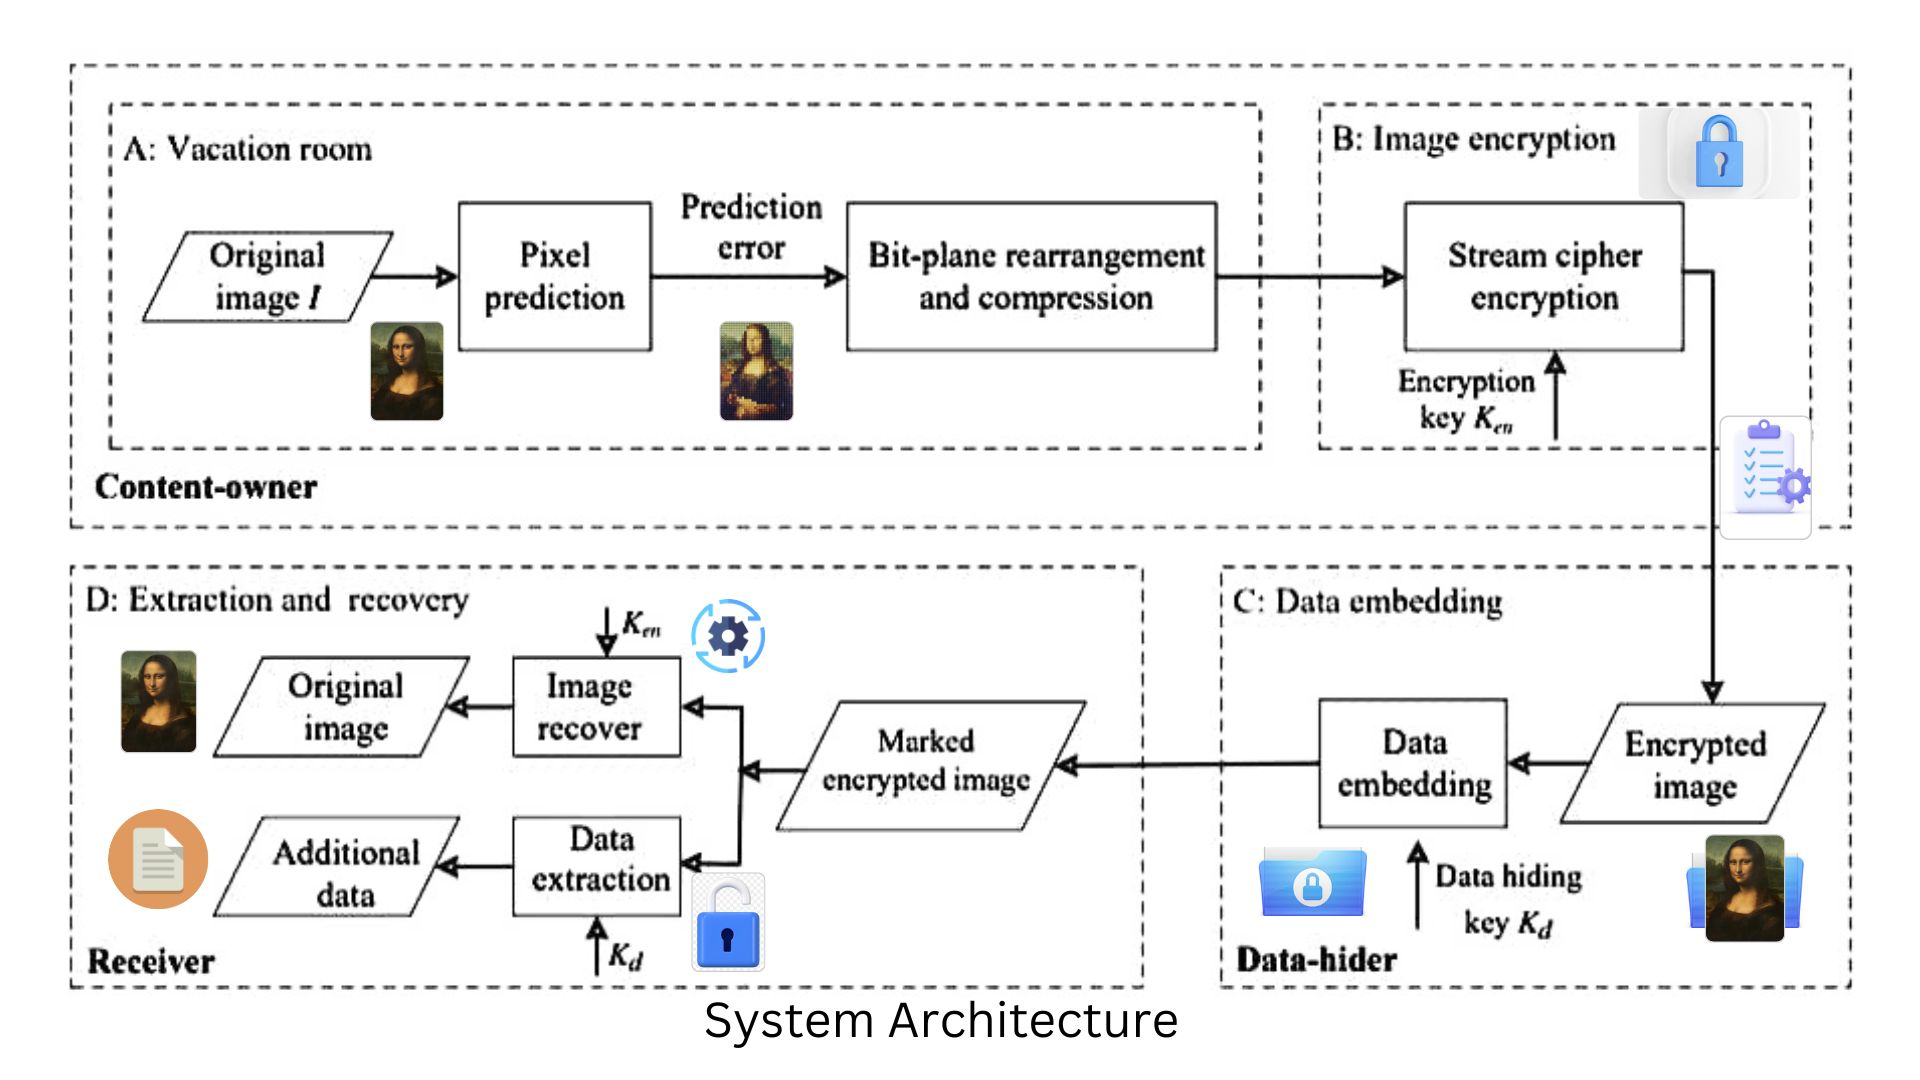
\includegraphics[height=6cm]{System Architecture.jpg}

\end{frame}


\section[Hardware and Software Requirements]{Hardware and Software Requirements}

\begin{frame}{Hardware and Software Requirements}
\begin{itemize}
        \item[1] \textbf{Hardware Requirement}
        \begin{itemize}
            \item i3 microprocessor based computer or higher
            \item memory
            \item Input/Output Interfaces
        \end{itemize}
        \item[2] \textbf{Software Requirement}
        \begin{itemize}
            \item Python libraries: openCV, Pillow, and scikit-image
            \item Steganography Libraries: OpenStego
            \item File Compression Software
            \item Version Control Software(Git)
            \item Image Editing Software
        \end{itemize}
\end{itemize}



\end{frame}


\section[Conclusion]{Conclusion}

\begin{frame}{Conclusion}
\begin{itemize}
    \item In conclusion, reversible data hiding with images is a complex endeavor that aims to securely embed confidential information while maintaining the image's integrity.

    \item  Striking the right balance between data capacity, minimal distortion, and resistance to attacks is key. 

    \item  As technology evolves, the pursuit of effective solutions continues to play a crucial role in securing digital information within the visual medium of images.
\end{itemize}
 

\end{frame}



\appendix

\begin{frame}[fragile]{} 
\begin{center}
    \textbf\Large{Thank You!}
\end{center}
\end{frame}

\end{document}
